\documentclass[../main.tex]{subfiles}
\graphicspath{ {images/Images/} }

\begin{document}
La detección de ondas sismológicas se encuentra en el núcleo de la sismología observacional hoy en día. Y es por esto que un buen algoritmo es aquel que es sensible a eventos fuertes y débiles, o con diferentes formas de la onda, además debe ser efectivo ante ruido en los datos y debe ser óptimo ante grandes volúmenes de datos. Se ha observado que en los últimos 10 años ha habido un incremento gigante en el volumen de datos sismológicos, se estima que cada año más de 50 terabytes se archivan a la incorporación de institutos para la investigación en sismología (IRIS). (Mousavi)\\

En general el desarollo de una CNN se da en tres etapas principalmente: pre-procesamiento de la señal, entrenamiento de la red y la arquitectura del algoritmo. Durante el entrenamiento los coeficientes de los filtros y los pesos de las capas conectadas completamente son optimizados. Este proceso puede verse como un sistema para extraer las características principales de los datos que se ingresan. En la arquitectura del algoritmo se encuentran las mayores diferencias entre los métodos usados actualmente, por lo que son variaciones que permiten modelar el problema según los objetivos establecidos por los autores.\\

\section{Etapas de la red}
\subsection{Pre-procesamiento de datos}

Es importante declarar en primer lugar que el pre-procesamiento de los datos en general es leve y puede jugar un papel importante en la efectividad del método. Algunos autores prefieren no realizar esta etapa, pero en general se normaliza cada componente removiendo la media y dividiendo por la desviación estándar. Además, se reduce la frecuencia de muestreo (decimate) para que la función quede de 100Hz como es el caso de Zhu. Pero existen ciertas variaciones que en algunas ocasiones se aplican, como por ejemplo Ross (2018)quien removía la media a los datos y aplicaba un filtro Butterworth pero sin remover la respuesta instrumental. En todo caso lo más común es normalizar y reducir la frecuencia de muestreo de los datos en cada componente.\\

\subsection{Entrenamiento de la red}

Para extraer las características principales de la señal de entrada es necesario entrenar la CNN. La calidad del entrenamiento también puede ayudar a acelerar la convergencia del algoritmo porque aumenta la información de las llegadas de ondas con respecto al ruido, así como información extra en la correlación temporal mejora los tiempos estimados para terremotos similares a los que se usan durante el entrenamiento.\\

Para la red PhaseNet, desarrollada por Zhu, se usaron datos analizados por el centro de datos sísmicos del norte de California (NCEDC) y se representaron las llegadas de las ondas P y S con distribuciones gaussianas con promedio cero y desviación de 0,1s. Estas representaciones reducen la influencia de los errores y sesgos de los sismólogos a la hora de detectar las ondas. Por su parte, Wu propone un entrenamiento en el cual se buscan relaciones entre eventos sísmicos y las señales que se evalúan mediante la correlación temporal. También hay autores que usan algoritmos de optimización estocásticos, como es el caso de Ross y Perol quienes usan un algoritmo llamado Adam.

\subsection{Arquitectura del algoritmo}

En su gran mayoría la estructura de los algoritmos es muy similar, aunque evidentemente difieren para cada caso. El patrón más característico es el de tener varios bloques de capas de convolución y de pooling, seguido de bloques de capas completamente conectadas que clasifican los valores de salida. En la figura 4.1 podemos observar un ejemplo de una estructura de la CNN correspondiente a Perol.  \\

\begin{figure}[h]
    \centering
    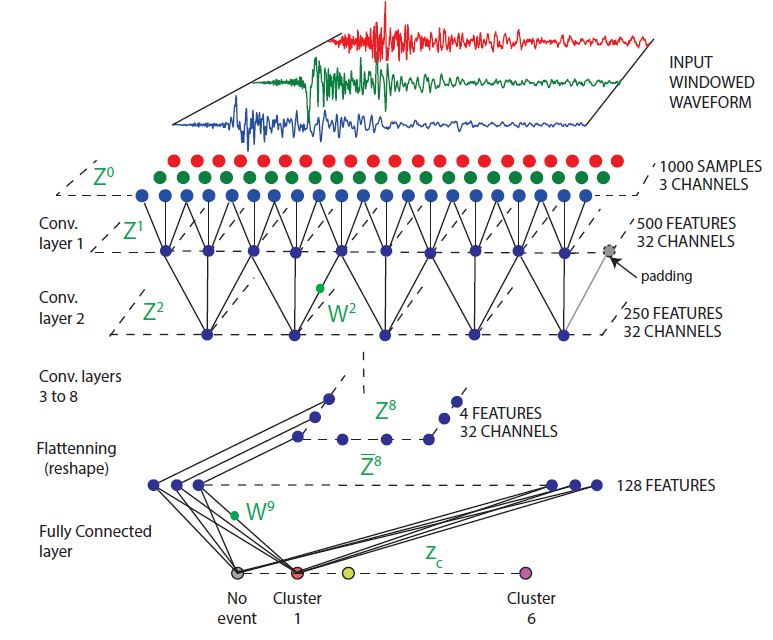
\includegraphics[width=0.5\textwidth]{RED.JPG}
    \label{fig:reda}
    \centering
    \caption{\centering La red recibe un sismograma de 3 componentes con 1000 muestras. Cada capa de convolución contiene 32 filtros que reducen los datos por un factor de 2. Luego de la capa 8 de convolución los resultados obtenidos se transforman en un vector 1D con 128 características. Finalmente se llega a una capa completamente conectada que arroja los resultados según las clases que haya. Tomado de Perol}
\end{figure}

La red de Perol recibe parámetros de entrada que pasan por una red compuesta de 8 capas de convolución seguida de una capa conectada completamente. Cada capa de convolución recibe los parámetros de salida de la anterior y les aplica una convolución con un filtro, cada resultado se suma y se le agrega un término de bias. A continuación se opera en una función no lineal de activación, ReLU, la cual es la más común. Este proceso se repite para cada capa con un stride de 2, lo que significa que el filtro hacia saltos dobles (en vez de simples). Luego de pasar por las capas de convolución, el ultimo resultado es procesado por una capa lineal completamente conectada y normalizado para finalmente obtener la clasificación. \\

PhaseNet recibe sismogramas de 3 componentes y los clasifica como onda P,S o ruido. Zhu usó diferentes SNR, los cuales se calculan como la proporción de las desviaciones estándar de los 5 segundos antes y después de la llegada P. Zhu propone un esquema de 9 bloques de convolución, en donde cada bloque consta de un proceso de convolución y activación. Durante los primeros 5 bloques se aplica un "stride" de 2, con filtros de 7x7 para reducir las dimensiones de los datos con el fin de extraer la información más importante. Durante los siguientes bloques se realiza un aumento de las dimensiones de los datos para expandir y convertir esa información en distribuciones probabilísticas. \\

Mousavi implemento un algoritmo con capas de convolución, recurrentes y conectadas completamente en una estructura residual. La estructura residual se refiere a que la red aprenderá las funciones residuales y no las funciones de clasificación (a diferencia del resto de autores acá citados). En primer lugar, durante un bloque de capas de convolución los autores le realizan una normalización a la función de activación de una capa. Esto acelera el entrenamiento y ayuda a prevenir el overfitting. A medida que el proceso se adentra en la red, estas capas van aprendiendo automáticamente de las características de los espectrogramas a niveles cada vez más detallados. Es importante notar que el autor interponía cada dos bloques de capas de convolución uno con un stride de 2, además que el número de filtros cada tres capas se duplicaba para preservar la complejidad temporal por capa.\\

Luego del bloque de capas de convolución sigue un bloque de capas recurrentes, donde los parámetros de entrada se distribuyen y pasan por dos capas bidireccionales seguidas de una capa unidireccional. La capa unidireccional se usa para ser consecuentes con la dirección en que los sismogramas incrementan temporalmente. Finalmente las ultimas dos capas de la red son capas conectadas completamente, cuyo resultado es un vector de probabilidades de contener una señal sismológica.\\


La red de convolución de Wu consta de 9 bloques de convolución y seis bloques de pooling. Cada bloque de convolución consta de 3 capas de convolución que luego seguirán un bloque de pooling donde se aplica una reducción en la dimensionalidad de la señal con una extra capa de convolución que reduce la dimensión de las características a la mitad. 


\section{Métodos de evaluación}

En la gran mayoría de los casos mencionados los autores presentan tres parámetros para evaluar el método propuesto; estas son: precisión, sensibilidad, F1. Las cuales se definen de la siguiente manera:\\

\begin{equation}
    precisión: P = \frac{T_p}{T_p + F_p}
\end{equation}
\begin{equation}
    Sensibilidad: R = \frac{T_p}{T_p + F_n}
\end{equation}
\begin{equation}
    F1 = 2\frac{P*R}{P + R}
\end{equation}

donde $T_p$ es el número de aciertos, $F_p$ es el número de falsos positivos, y $F_n$ es el número de falsos negativos. El escenario ideal para un algoritmo es tener una precisión y sensibilidad alta, es decir cercana a 1. Mientras que el parámetro F1 representa la importancia que tiene la precisión y sensibilidad en el algoritmo, es decir que es una forma de cuantificar el valor de una con respecto a la otra. \\




\end{document} 